% -*- mode: latex; mode: flyspell; ispell-local-dictionary: "en_US"; coding: utf-8 -*-

\documentclass{standalone}

\usepackage[utf8]{inputenc}
\usepackage[english]{babel}

\usepackage{amsmath,amsfonts,amssymb}

\usepackage{tikz,pgfplots}
\usetikzlibrary{plotmarks}
\pgfplotsset{compat=newest}

\usepgfplotslibrary{groupplots}
\pgfplotsset{every axis/.style={scale only axis}}

\pgfplotsset{
  major grid style={dashed},
  minor grid style={thin,dotted},
  ymajorgrids,
  yminorgrids,
  every axis/.append style={
    line width=0.7pt,
    tick style={
      line cap=round,
      thin,
      major tick length=4pt,
      minor tick length=2pt,
    },
  },
  legend cell align=left,
  legend style={
    line width=0.7pt,
    /tikz/every even column/.append style={column sep=3mm,black},
    /tikz/every odd column/.append style={black},
  },
  % move title closer
  legend style={font=\small},
  title style={yshift=-2pt},
  % less space on left and right
  enlarge x limits=0.04,
  every tick label/.append style={font=\footnotesize},
  every axis label/.append style={font=\small},
  every axis y label/.append style={yshift=-1ex},
  /pgf/number format/1000 sep={},
  axis lines*=left,
  xlabel near ticks,
  ylabel near ticks,
  axis lines*=left,
  label style={font=\footnotesize},       
  tick label style={font=\footnotesize},
  plotConstruction/.style={
    width=38mm,
    height=38mm,
    only marks,
    ymin=9,
    ymax=2000,
  },
}


\usepackage{xcolor}
\definecolor{my-dark-red}{RGB}{183, 28, 28}
\definecolor{my-red}{RGB}{244,67,54}
\definecolor{my-pink}{RGB}{233,30,99}
\definecolor{my-purple}{RGB}{156,39,176}
\definecolor{my-deep-purple}{RGB}{103,58,183}
\definecolor{my-indigo}{RGB}{63,81,181}
\definecolor{my-blue}{RGB}{33,150,243}
\definecolor{my-light-blue}{RGB}{3,169,244}
\definecolor{my-cyan}{RGB}{0,188,212}
\definecolor{my-teal}{RGB}{0,150,136}
\definecolor{my-green}{RGB}{76,175,80}
\definecolor{my-light-green}{RGB}{139,195,74}
\definecolor{my-lime}{RGB}{205,220,57}
\definecolor{my-yellow}{RGB}{255,235,59}
\definecolor{my-amber}{RGB}{255,193,7}
\definecolor{my-orange}{RGB}{255,152,0}
\definecolor{my-deep-orange}{RGB}{255,87,34}
\definecolor{my-brown}{RGB}{121,85,72}
\definecolor{my-grey}{RGB}{158,158,158}
\definecolor{my-blue-grey}{RGB}{96,125,139}
\definecolor{my-lipics-grey}{rgb}{0.6,0.6,0.61}


\colorlet{fp1Color}{my-blue}
\colorlet{fpzColor}{my-blue}
\colorlet{lpf1Color}{my-green}
\colorlet{lpfzColor}{my-green}
\colorlet{lpf1dpColor}{my-deep-orange}
\colorlet{lpfzdpColor}{my-deep-orange}
\colorlet{belazzouguiColor}{my-dark-red}

\begin{document}

% IMPORT-DATA our_stats ./data/repetitive_our.txt
% IMPORT-DATA belazzougui_stats ./data/repetitive_belazzougui.txt
% IMPORT-DATA algorithm_meta_data ./data/algorithm_names.txt

%% SQL DELETE FROM our_stats WHERE algorithm LIKE 'FP-pruning-z'

\begin{tabular}{lll}
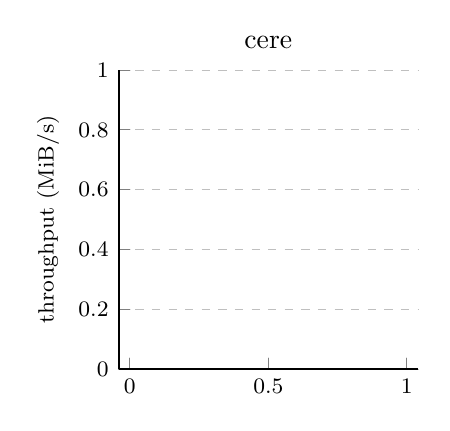
\begin{tikzpicture}
\begin{axis}[
  title={cere},
  ylabel={throughput (MiB/s)},
  %ymode=log,
  plotConstruction,
  legend to name={leg:construction_with_rs}
]
%% MULTIPLOT(algorithm|attr|ptitle)
%% SELECT (space_usage_with_rs*8.0)/prefix_size AS x, (prefix_size/1024.0/1024.0)/AVG(construction_time_with_rs_ms/1000.0) AS y, plot_attr AS attr, plot_name AS ptitle, MULTIPLOT
%% FROM our_stats
%% JOIN algorithm_meta_data ON algorithm = algorithm_name
%% WHERE input LIKE '%cere%'
%%GROUP BY MULTIPLOT,x ORDER BY sorting_order
\addplot[mark=asterisk,color=fp1Color] coordinates { (0.644678,0.420089) (0.64978,0.836572) (0.723432,0.40326) (0.773795,1.13554) (0.788928,0.768653) (0.879139,1.69312) (0.895879,0.388331) (0.902253,0.384861) (1.20825,0.746788) (1.23451,1.00337) (1.37357,1.35793) };
\addlegendentry{FP$_1$};
\addplot[mark=triangle,color=lpfzColor] coordinates { (0.748612,4.63891) (0.870664,4.52751) (0.887851,4.4667) (0.892087,4.66703) (0.949405,4.43429) (1.01153,4.59427) (1.12185,4.16792) (1.12823,3.97086) (1.30719,4.12506) (1.38658,4.23849) (1.47603,4.08753) };
\addlegendentry{LPF$_z$};
\addplot[mark=pentagon,color=lpfzdpColor] coordinates { (0.748612,4.51659) (0.870664,4.39456) (0.887851,4.34441) (0.892087,4.57139) (0.949405,4.27554) (1.01153,4.51163) (1.12185,4.08751) (1.12823,3.94375) (1.30719,4.106) (1.38658,4.19186) (1.47603,4.10802) };
\addlegendentry{LPF$^{\textnormal{DP}}_z$};
\addplot[mark=x,color=lpf1dpColor] coordinates { (0.644678,3.75779) (0.64978,4.14926) (0.723432,3.70223) (0.773795,4.25155) (0.788928,4.00823) (0.879139,4.34403) (0.895879,3.56328) (0.902253,3.4698) (1.20825,3.79499) (1.23451,3.91953) (1.37357,4.02243) };
\addlegendentry{LPF$^{\textnormal{DP}}_1$};
\addplot[mark=+,color=lpf1Color] coordinates { (0.644678,4.46746) (0.64978,4.56246) (0.723432,4.37457) (0.773795,4.49703) (0.788928,4.38154) (0.879139,4.59986) (0.895879,4.13231) (0.902253,3.92745) (1.20825,4.02912) (1.23451,3.98265) (1.37357,4.13404) };
\addlegendentry{LPF$_1$};

%% MULTIPLOT(algorithm|attr|ptitle)
%% SELECT (space_usage_with_rs*8.0)/prefix_size AS x,(prefix_size/1024.0/1024.0)/AVG(construction_time_with_rs/1000.0) AS y, plot_attr AS attr, plot_name AS ptitle, sorting_order AS sorting_order, MULTIPLOT
%% FROM belazzougui_stats
%% JOIN algorithm_meta_data ON algorithm = algorithm_name
%% WHERE input LIKE '%cere%'
%%GROUP BY MULTIPLOT,x ORDER BY MULTIPLOT,x
\addplot[mark=star,color=belazzouguiColor,scale=.9] coordinates { (0.646644,0.455588) (0.651082,0.850894) (0.726099,0.444699) (0.775276,1.10199) (0.791307,0.793694) (0.795555,0.801421) (0.860785,1.1921) (0.87987,1.54067) (0.899612,0.430491) (1.18445,1.07159) (1.33583,1.29488) (1.39909,1.3724) };
\addlegendentry{original~BT~\cite{belazzougui21block}};

\end{axis}
\end{tikzpicture}
  &
    \begin{tikzpicture}
\begin{axis}[
  title={coreutils},
  %ymode=log,
  ymajorticks=false,
  plotConstruction,
]
%% MULTIPLOT(algorithm|attr|ptitle)
%% SELECT (space_usage_with_rs*8.0)/prefix_size AS x, (prefix_size/1024.0/1024.0)/AVG(construction_time_with_rs_ms/1000.0) AS y, plot_attr AS attr, plot_name AS ptitle, sorting_order AS sorting_order, MULTIPLOT
%% FROM our_stats
%% JOIN algorithm_meta_data ON algorithm = algorithm_name
%% WHERE input LIKE '%coreutils%'
%%GROUP BY MULTIPLOT,x ORDER BY sorting_order
\addplot[mark=asterisk,color=fp1Color] coordinates { (5.7661,1.79944) (8.88095,0.889904) (9.7985,1.17706) (13.5657,0.456582) (17.63,0.638864) (18.564,0.399951) (24.8503,0.336014) (25.598,0.780857) (29.0327,0.593831) (30.9062,0.279084) (32.1765,0.411634) };
\addlegendentry{FP$_1$};
\addplot[mark=triangle,color=lpfzColor] coordinates { (18.0339,2.04881) (20.8591,2.63876) (25.6662,1.8055) (29.4324,1.24172) (34.4295,0.894933) (34.6046,0.990067) (37.5281,0.748954) (40.7153,0.616119) (43.3189,0.859068) (46.7712,0.437378) (49.1822,0.507991) };
\addlegendentry{LPF$_z$};
\addplot[mark=pentagon,color=lpfzdpColor] coordinates { (18.0339,2.01438) (20.8591,2.60013) (25.6662,1.77818) (29.4324,1.22374) (34.4295,0.884284) (34.6046,0.976521) (37.5281,0.742958) (40.7153,0.612409) (43.3189,0.847766) (46.7712,0.435418) (49.1822,0.506254) };g
\addlegendentry{LPF$^{\textnormal{DP}}_z$};
\addplot[mark=x,color=lpf1dpColor] coordinates { (5.7661,3.84976) (8.88095,2.78495) (9.7985,2.59904) (13.5657,1.86481) (17.63,1.42134) (18.564,1.30433) (24.8503,0.860817) (25.598,1.13455) (29.0327,0.885549) (30.9062,0.581757) (32.1765,0.661829) };
\addlegendentry{LPF$^{\textnormal{DP}}_1$};
\addplot[mark=+,color=lpf1Color] coordinates { (5.7661,4.03606) (8.88095,2.96072) (9.7985,2.72521) (13.5657,2.00648) (17.63,1.4717) (18.564,1.37436) (24.8503,0.885324) (25.598,1.15928) (29.0327,0.897215) (30.9062,0.591426) (32.1765,0.668378) };
\addlegendentry{LPF$_1$};

%% MULTIPLOT(algorithm|attr|ptitle)
%% SELECT (space_usage_with_rs*8.0)/prefix_size AS x, (prefix_size/1024.0/1024.0)/AVG(construction_time_with_rs/1000.0) AS y, plot_attr AS attr, plot_name AS ptitle, sorting_order AS sorting_order, MULTIPLOT
%% FROM belazzougui_stats
%% JOIN algorithm_meta_data ON algorithm = algorithm_name
%% WHERE input LIKE '%coreutils%'
%%GROUP BY MULTIPLOT,x ORDER BY MULTIPLOT,x
\addplot[mark=star,color=belazzouguiColor,scale=.9] coordinates { (5.76662,0.359367) (8.8822,0.308075) (9.79978,0.24082) (10.0858,0.364589) (13.5782,0.198259) (17.6332,0.14693) (17.7996,0.211223) (18.5678,0.142669) (24.8558,0.101692) (25.9307,0.157208) (26.2138,0.243166) (29.247,0.159667) };
\addlegendentry{original~BT~\cite{belazzougui21block}};

\legend{};

\end{axis}
\end{tikzpicture}
  &
    \hspace{.5cm}
    \raisebox{1cm}{\ref*{leg:construction_with_rs}}
  \\
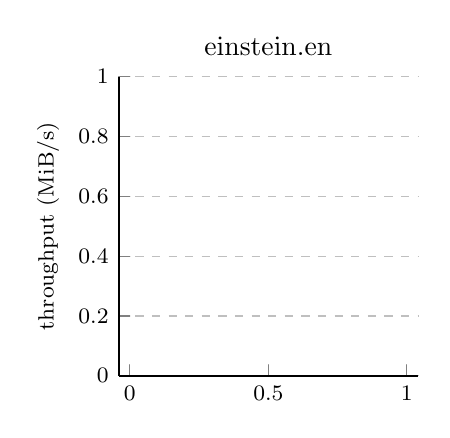
\begin{tikzpicture}
\begin{axis}[
  title={einstein.en},
  ylabel={throughput (MiB/s)},
  %ymode=log,
  plotConstruction,
]
%% MULTIPLOT(algorithm|attr|ptitle)
%% SELECT (space_usage_with_rs*8.0)/prefix_size AS x, (prefix_size/1024.0/1024.0)/AVG(construction_time_with_rs_ms/1000.0) AS y, plot_attr AS attr, plot_name AS ptitle, sorting_order AS sorting_order, MULTIPLOT
%% FROM our_stats
%% JOIN algorithm_meta_data ON algorithm = algorithm_name
%% WHERE input LIKE '%einstein.en.txt%'
%%GROUP BY MULTIPLOT,x ORDER BY sorting_order
\addplot[mark=asterisk,color=fp1Color] coordinates { (0.516775,1.13299) (0.517796,0.579684) (0.580855,0.566242) (0.632242,1.08393) (0.665634,0.553125) (0.68349,1.52299) (0.766803,0.54141) (0.820173,2.13481) (0.836285,1.03204) (0.949648,1.40068) (1.23407,1.89039) };
\addlegendentry{FP$_1$};
\addplot[mark=triangle,color=lpfzColor] coordinates { (0.593785,4.20142) (0.706611,4.11788) (0.709275,4.03497) (0.733992,4.02277) (0.797037,3.92885) (0.820173,4.14146) (0.88183,3.80679) (0.913306,3.77977) (0.972769,3.80672) (0.983001,3.66507) (1.23407,3.67058) };
\addlegendentry{LPF$_z$};
\addplot[mark=pentagon,color=lpfzdpColor] coordinates { (0.593785,4.15843) (0.706611,4.0631) (0.709275,3.98982) (0.733992,3.98453) (0.797037,3.87241) (0.820173,4.0933) (0.88183,3.77477) (0.913306,3.76468) (0.972769,3.76889) (0.983001,3.61966) (1.23407,3.64177) };g
\addlegendentry{LPF$^{\textnormal{DP}}_z$};
\addplot[mark=x,color=lpf1dpColor] coordinates { (0.516775,3.99354) (0.517796,3.78643) (0.580855,3.7115) (0.632242,3.84008) (0.665634,3.61874) (0.68349,3.95127) (0.766803,3.50999) (0.820173,3.99373) (0.836285,3.63605) (0.949648,3.66675) (1.23407,3.5628) };
\addlegendentry{LPF$^{\textnormal{DP}}_1$};
\addplot[mark=+,color=lpf1Color] coordinates { (0.516775,4.23506) (0.517796,4.16756) (0.580855,4.08041) (0.632242,4.05859) (0.665634,3.97098) (0.68349,4.11486) (0.766803,3.82524) (0.820173,4.14151) (0.836285,3.82969) (0.949648,3.8032) (1.23407,3.67228) };
\addlegendentry{LPF$_1$};

%% MULTIPLOT(algorithm|attr|ptitle)
%% SELECT (space_usage_with_rs*8.0)/prefix_size AS x, (prefix_size/1024.0/1024.0)/AVG(construction_time_with_rs/1000.0) AS y, plot_attr AS attr, plot_name AS ptitle, sorting_order AS sorting_order, MULTIPLOT
%% FROM belazzougui_stats
%% JOIN algorithm_meta_data ON algorithm = algorithm_name
%% WHERE input LIKE '%einstein.en.txt%'
%%GROUP BY MULTIPLOT,x ORDER BY MULTIPLOT,x
\addplot[mark=star,color=belazzouguiColor,scale=.9] coordinates { (0.516894,1.17287) (0.51792,0.659286) (0.581008,0.643977) (0.632407,1.08224) (0.636182,1.11427) (0.665828,0.622584) (0.683641,1.41249) (0.697523,1.52335) (0.820326,1.686) (0.954829,1.36204) (1.24276,1.4525) (1.25637,1.53306) };
\addlegendentry{original~BT~\cite{belazzougui21block}};

\legend{};

\end{axis}
\end{tikzpicture}
  &
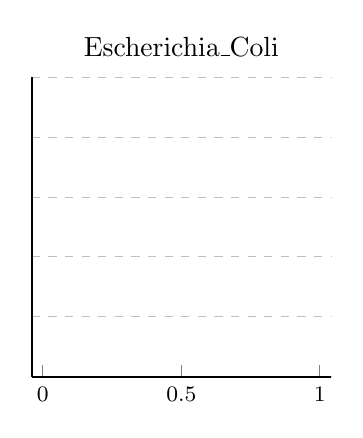
\begin{tikzpicture}
\begin{axis}[
  title={Escherichia\_Coli},
  ymajorticks=false,
  %ymode=log,
  plotConstruction,
]
%% MULTIPLOT(algorithm|attr|ptitle)
%% SELECT (space_usage_with_rs*8.0)/prefix_size AS x, (prefix_size/1024.0/1024.0)/AVG(construction_time_with_rs_ms/1000.0) AS y, plot_attr AS attr, plot_name AS ptitle, sorting_order AS sorting_order, MULTIPLOT
%% FROM our_stats
%% JOIN algorithm_meta_data ON algorithm = algorithm_name
%% WHERE input LIKE '%Escherichia_Coli%'
%%GROUP BY MULTIPLOT,x ORDER BY sorting_order
\addplot[mark=asterisk,color=fp1Color] coordinates { (2.41235,0.86433) (2.49111,1.80375) (2.51002,1.20225) (2.96602,0.424271) (3.51367,0.707105) (3.69099,0.387056) (4.60391,1.14332) (5.0389,0.352237) (5.07664,0.339276) (5.50772,0.862642) (6.88379,0.627397) };
\addlegendentry{FP$_1$};
\addplot[mark=triangle,color=lpfzColor] coordinates { (2.9873,4.84073) (4.99421,4.26981) (5.13347,3.30902) (5.4074,3.81461) (6.13613,3.27191) (6.17168,3.37507) (7.48483,2.24438) (7.52256,1.78816) (8.17032,2.32579) (9.5633,2.0346) };
\addlegendentry{LPF$_z$};
\addplot[mark=pentagon,color=lpfzdpColor] coordinates { (2.9873,4.67142) (4.99421,4.13553) (5.13347,3.18268) (5.4074,3.63616) (6.13613,3.09035) (6.17168,3.22219) (7.48483,2.22589) (7.52256,1.85144) (8.17032,2.4041) (9.5633,2.08388) };
\addlegendentry{LPF$^{\textnormal{DP}}_z$};
\addplot[mark=x,color=lpf1dpColor] coordinates { (2.41235,3.70882) (2.49111,4.28819) (2.51002,3.85609) (2.96602,2.92773) (3.51367,3.03589) (3.69099,2.63806) (4.60391,3.01654) (5.0389,2.05852) (5.07664,1.78084) (5.50772,2.42585) (6.88379,2.10139) };
\addlegendentry{LPF$^{\textnormal{DP}}_1$};
\addplot[mark=+,color=lpf1Color] coordinates { (2.41235,4.57971) (2.49111,4.88215) (2.51002,4.50041) (2.96602,4.06177) (3.51367,3.66274) (3.69099,3.54512) (4.60391,3.36096) (5.0389,2.48671) (5.07664,1.98978) (5.50772,2.5175) (6.88379,2.23551) };
\addlegendentry{LPF$_1$};

%% MULTIPLOT(algorithm|attr|ptitle)
%% SELECT (space_usage_with_rs*8.0)/prefix_size AS x, (prefix_size/1024.0/1024.0)/AVG(construction_time_with_rs/1000.0) AS y, plot_attr AS attr, plot_name AS ptitle, sorting_order AS sorting_order, MULTIPLOT
%% FROM belazzougui_stats
%% JOIN algorithm_meta_data ON algorithm = algorithm_name
%% WHERE input LIKE '%Escherichia_Coli%'
%%GROUP BY MULTIPLOT,x ORDER BY MULTIPLOT,x
\addplot[mark=star,color=belazzouguiColor,scale=.9] coordinates { (2.41524,0.750315) (2.49198,1.42368) (2.51283,0.916834) (2.8059,1.09741) (2.97216,0.38978) (3.52147,0.52238) (3.59197,0.627925) (3.70082,0.339028) (4.69979,0.897873) (4.97575,1.16843) (5.05455,0.267224) (5.58203,0.730066) };
\addlegendentry{original~BT~\cite{belazzougui21block}};

\legend{};

\end{axis}
\end{tikzpicture}
  &
\begin{tikzpicture}
\begin{axis}[
  title={influenza},
  %ymode=log,
  ymajorticks=false,
  plotConstruction,
]
%% MULTIPLOT(algorithm|attr|ptitle)
%% SELECT (space_usage_with_rs*8.0)/prefix_size AS x, (prefix_size/1024.0/1024.0)/AVG(construction_time_with_rs_ms/1000.0) AS y, plot_attr AS attr, plot_name AS ptitle, sorting_order AS sorting_order, MULTIPLOT
%% FROM our_stats
%% JOIN algorithm_meta_data ON algorithm = algorithm_name
%% WHERE input LIKE '%influenza%'
%%GROUP BY MULTIPLOT,x ORDER BY sorting_order
\addplot[mark=asterisk,color=fp1Color] coordinates { (1.74031,0.793446) (1.75293,0.407202) (1.92742,0.392264) (1.9786,1.13459) (2.10721,0.380767) (2.13343,0.717565) (2.13494,0.373227) (2.24299,1.64175) (2.61375,0.681186) (3.30433,0.963997) (3.63195,1.22128) };
\addlegendentry{FP$_1$};
\addplot[mark=triangle,color=lpfzColor] coordinates { (2.14243,4.38834) (2.16131,3.95937) (2.18911,4.47213) (2.3357,3.49798) (2.51549,3.04314) (2.54322,2.7817) (2.58724,3.58003) (2.61542,4.90749) (3.06765,2.94508) (3.46842,2.99399) (4.00606,3.20527) };
\addlegendentry{LPF$_z$};
\addplot[mark=pentagon,color=lpfzdpColor] coordinates { (2.14243,4.31359) (2.16131,3.85388) (2.18911,4.37154) (2.3357,3.44257) (2.51549,3.01976) (2.54322,2.79688) (2.58724,3.55177) (2.61542,4.80589) (3.06765,2.99327) (3.46842,3.0685) (4.00606,3.22862) };g
\addlegendentry{LPF$^{\textnormal{DP}}_z$};
\addplot[mark=x,color=lpf1dpColor] coordinates { (1.74031,3.98602) (1.75293,3.29343) (1.92742,3.0066) (1.9786,3.99943) (2.10721,2.70677) (2.13343,3.30923) (2.13494,2.53273) (2.24299,4.52707) (2.61375,2.82808) (3.30433,2.92722) (3.63195,3.06445) };
\addlegendentry{LPF$^{\textnormal{DP}}_1$};
\addplot[mark=+,color=lpf1Color] coordinates { (1.74031,4.47602) (1.75293,3.9774) (1.92742,3.51427) (1.9786,4.35691) (2.10721,3.07855) (2.13343,3.59717) (2.13494,2.81917) (2.24299,4.87841) (2.61375,2.9619) (3.30433,2.99982) (3.63195,3.14213) };
\addlegendentry{LPF$_1$};

%% MULTIPLOT(algorithm|attr|ptitle)
%% SELECT (space_usage_with_rs*8.0)/prefix_size AS x, (prefix_size/1024.0/1024.0)/AVG(construction_time_with_rs/1000.0) AS y, plot_attr AS attr, plot_name AS ptitle, sorting_order AS sorting_order, MULTIPLOT
%% FROM belazzougui_stats
%% JOIN algorithm_meta_data ON algorithm = algorithm_name
%% WHERE input LIKE '%influenza%'
%%GROUP BY MULTIPLOT,x ORDER BY MULTIPLOT,x
\addplot[mark=star,color=belazzouguiColor,scale=.9] coordinates { (1.74301,0.700214) (1.7572,0.376891) (1.93274,0.352104) (1.98149,0.879013) (2.11335,0.327763) (2.13846,0.571191) (2.20858,0.633644) (2.24403,1.30717) (2.3482,1.05003) (3.24144,0.768882) (3.69744,0.932022) (4.02874,1.13701) };
\addlegendentry{original~BT~\cite{belazzougui21block}};

\legend{};

\end{axis}
\end{tikzpicture}
  \\
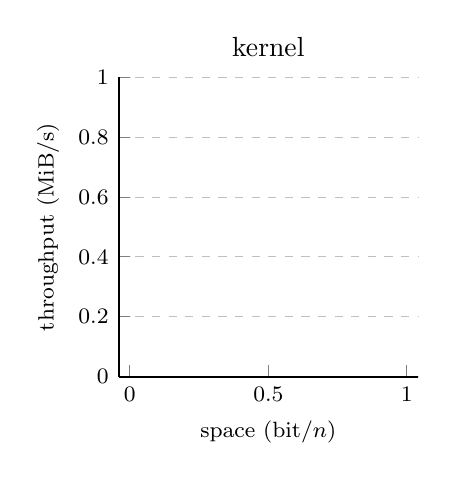
\begin{tikzpicture}
\begin{axis}[
  title={kernel},
  xlabel={space (\(\textnormal{bit}/n\))},
  ylabel={throughput (MiB/s)},
  %ymode=log,
  plotConstruction,
]
%% MULTIPLOT(algorithm|attr|ptitle)
%% SELECT (space_usage_with_rs*8.0)/prefix_size AS x, (prefix_size/1024.0/1024.0)/AVG(construction_time_with_rs_ms/1000.0) AS y, plot_attr AS attr, plot_name AS ptitle, sorting_order AS sorting_order, MULTIPLOT
%% FROM our_stats
%% JOIN algorithm_meta_data ON algorithm = algorithm_name
%% WHERE input LIKE '%kernel%'
%%GROUP BY MULTIPLOT,x ORDER BY sorting_order
\addplot[mark=asterisk,color=fp1Color] coordinates { (1.79396,2.26958) (1.84993,1.18846) (2.17508,1.64963) (2.60341,0.615662) (3.37459,1.03025) (3.69428,0.577716) (4.88638,1.55207) (5.38974,0.525466) (5.74957,1.18081) (7.19893,0.472398) (7.4392,0.805314) };
\addlegendentry{FP$_1$};
\addplot[mark=triangle,color=lpfzColor] coordinates { (2.3427,4.36221) (4.52282,3.51835) (5.45709,2.72679) (6.05261,2.68145) (7.53404,2.97918) (7.97314,2.49385) (9.06406,2.06456) (10.1188,1.54932) (10.7594,1.53622) (11.165,1.69772) (12.5686,1.12916) };
\addlegendentry{LPF$_z$};
\addplot[mark=pentagon,color=lpfzdpColor] coordinates { (2.3427,4.29834) (4.52282,3.4683) (5.45709,2.68102) (6.05261,2.63728) (7.53404,2.9352) (7.97314,2.45816) (9.06406,2.03443) (10.1188,1.53625) (10.7594,1.52304) (11.165,1.67696) (12.5686,1.12567) };g
\addlegendentry{LPF$^{\textnormal{DP}}_z$};
\addplot[mark=x,color=lpf1dpColor] coordinates { (1.79396,4.37141) (1.84993,4.10605) (2.17508,3.95596) (2.60341,3.5104) (3.37459,3.17141) (3.69428,2.97702) (4.88638,2.73916) (5.38974,2.23317) (5.74957,2.33509) (7.19893,1.62772) (7.4392,1.83497) };
\addlegendentry{LPF$^{\textnormal{DP}}_1$};
\addplot[mark=+,color=lpf1Color] coordinates { (1.79396,4.57347) (1.84993,4.38718) (2.17508,4.18569) (2.60341,3.8892) (3.37459,3.36256) (3.69428,3.25515) (4.88638,2.83139) (5.38974,2.39878) (5.74957,2.41893) (7.19893,1.69555) (7.4392,1.89289) };
\addlegendentry{LPF$_1$};

%% MULTIPLOT(algorithm|attr|ptitle)
%% SELECT (space_usage_with_rs*8.0)/prefix_size AS x, (prefix_size/1024.0/1024.0)/AVG(construction_time_with_rs/1000.0) AS y, plot_attr AS attr, plot_name AS ptitle, sorting_order AS sorting_order, MULTIPLOT
%% FROM belazzougui_stats
%% JOIN algorithm_meta_data ON algorithm = algorithm_name
%% WHERE input LIKE '%kernel%'
%%GROUP BY MULTIPLOT,x ORDER BY MULTIPLOT,x
\addplot[mark=star,color=belazzouguiColor,scale=.9] coordinates { (1.79423,0.921076) (1.85037,0.772219) (2.17557,0.706269) (2.23382,0.919747) (2.60424,0.473697) (3.37569,0.451947) (3.42637,0.607114) (3.69565,0.37983) (4.96915,0.501148) (5.02895,0.708463) (5.39194,0.283097) (5.84364,0.509048) };
\addlegendentry{original~BT~\cite{belazzougui21block}};

\legend{};

\end{axis}
\end{tikzpicture}
  &
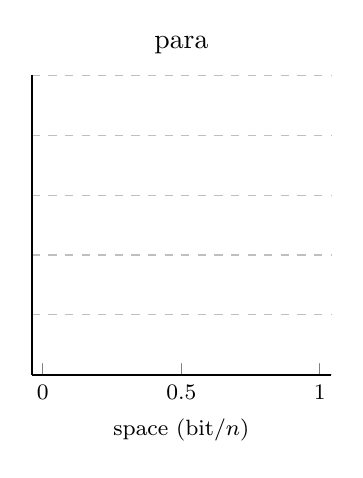
\begin{tikzpicture}
\begin{axis}[
  title={para},
  xlabel={space (\(\textnormal{bit}/n\))},
  %ymode=log,
  ymajorticks=false,
  plotConstruction,
]
%% MULTIPLOT(algorithm|attr|ptitle)
%% SELECT (space_usage_with_rs*8.0)/prefix_size AS x, (prefix_size/1024.0/1024.0)/AVG(construction_time_with_rs_ms/1000.0) AS y, plot_attr AS attr, plot_name AS ptitle, sorting_order AS sorting_order, MULTIPLOT
%% FROM our_stats
%% JOIN algorithm_meta_data ON algorithm = algorithm_name
%% WHERE input LIKE '%para%'
%%GROUP BY MULTIPLOT,x ORDER BY sorting_order
\addplot[mark=asterisk,color=fp1Color] coordinates { (0.766932,0.817092) (0.810071,0.404103) (0.889904,1.11427) (0.938086,0.383085) (0.98178,0.736568) (0.985833,1.68658) (1.21374,0.367025) (1.22217,0.36304) (1.53238,1.3141) (1.57869,0.963391) (1.66085,0.71154) };
\addlegendentry{FP$_1$};
\addplot[mark=triangle,color=lpfzColor] coordinates { (1.07578,4.56169) (1.29014,4.56673) (1.32772,4.43641) (1.37474,4.62632) (1.4557,4.28638) (1.50632,4.31289) (1.73135,3.90823) (1.73978,3.6427) (1.76609,3.91302) (1.9284,4.19844) (2.18616,3.81676) };
\addlegendentry{LPF$_z$};
\addplot[mark=pentagon,color=lpfzdpColor] coordinates { (1.07578,4.45019) (1.29014,4.45212) (1.32772,4.286) (1.37474,4.54654) (1.4557,4.12939) (1.50632,4.19106) (1.73135,3.85422) (1.73978,3.68626) (1.76609,3.97747) (1.9284,4.09996) (2.18616,3.85429) };g
\addlegendentry{LPF$^{\textnormal{DP}}_z$};
\addplot[mark=x,color=lpf1dpColor] coordinates { (0.766932,4.05246) (0.810071,3.61762) (0.889904,4.14223) (0.938086,3.5122) (0.98178,3.85423) (0.985833,4.27289) (1.21374,3.33986) (1.22217,3.22741) (1.53238,3.89567) (1.57869,3.74593) (1.66085,3.58878) };
\addlegendentry{LPF$^{\textnormal{DP}}_1$};
\addplot[mark=+,color=lpf1Color] coordinates { (0.766932,4.59988) (0.810071,4.48565) (0.889904,4.54475) (0.938086,4.32529) (0.98178,4.35655) (0.985833,4.6196) (1.21374,3.99261) (1.22217,3.71295) (1.53238,4.17178) (1.57869,3.9035) (1.66085,3.8511) };
\addlegendentry{LPF$_1$};

%% MULTIPLOT(algorithm|attr|ptitle)
%% SELECT (space_usage_with_rs*8.0)/prefix_size AS x, (prefix_size/1024.0/1024.0)/AVG(construction_time_with_rs/1000.0) AS y, plot_attr AS attr, plot_name AS ptitle, sorting_order AS sorting_order, MULTIPLOT
%% FROM belazzougui_stats
%% JOIN algorithm_meta_data ON algorithm = algorithm_name
%% WHERE input LIKE '%para%'
%%GROUP BY MULTIPLOT,x ORDER BY MULTIPLOT,x
\addplot[mark=star,color=belazzouguiColor,scale=.9] coordinates { (0.768367,0.823014) (0.812556,0.433017) (0.891476,1.07318) (0.941716,0.41694) (0.977558,1.16213) (0.984854,0.746271) (0.986651,1.50063) (0.993811,0.760649) (1.219,0.398059) (1.50175,1.01736) (1.51724,1.24863) (1.58772,1.30592) };
\addlegendentry{original~BT~\cite{belazzougui21block}};

\legend{};

\end{axis}
\end{tikzpicture}
  &
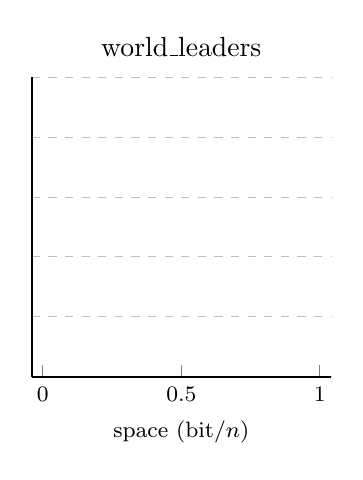
\begin{tikzpicture}
\begin{axis}[
  title={world\_leaders},
  xlabel={space (\(\textnormal{bit}/n\))},
  %ymode=log,
  ymajorticks=false,
  plotConstruction,
]
%% MULTIPLOT(algorithm|attr|ptitle)
%% SELECT (space_usage_with_rs*8.0)/prefix_size AS x, (prefix_size/1024.0/1024.0)/AVG(construction_time_with_rs_ms/1000.0) AS y, plot_attr AS attr, plot_name AS ptitle, sorting_order AS sorting_order, MULTIPLOT
%% FROM our_stats
%% JOIN algorithm_meta_data ON algorithm = algorithm_name
%% WHERE input LIKE '%world_leaders%'
%%GROUP BY MULTIPLOT,x ORDER BY sorting_order
\addplot[mark=asterisk,color=fp1Color] coordinates { (4.48835,1.90549) (4.58143,0.998047) (5.1717,0.532558) (5.50606,1.30213) (5.971,0.506424) (6.34727,0.856816) (6.84739,0.477685) (7.80956,0.449432) (8.60628,0.725797) (9.62151,0.946577) (11.2416,1.14003) };
\addlegendentry{FP$_1$};
\addplot[mark=triangle,color=lpfzColor] coordinates { (4.61565,4.33698) (5.36649,3.50232) (6.9111,2.7114) (7.13339,2.4561) (7.31247,3.22646) (7.70994,2.2614) (8.58642,1.86267) (9.39251,1.68945) (9.54863,1.54137) (11.37,1.88465) (11.4476,1.78699) };
\addlegendentry{LPF$_z$};
\addplot[mark=pentagon,color=lpfzdpColor] coordinates { (4.61565,4.26404) (5.36649,3.45558) (6.9111,2.66965) (7.13339,2.43091) (7.31247,3.17549) (7.70994,2.23262) (8.58642,1.85225) (9.39251,1.67646) (9.54863,1.53547) (11.37,1.86861) (11.4476,1.76949) };g
\addlegendentry{LPF$^{\textnormal{DP}}_z$};
\addplot[mark=x,color=lpf1dpColor] coordinates { (4.48835,4.11846) (4.58143,3.38387) (5.1717,2.72156) (5.50606,3.1969) (5.971,2.29956) (6.34727,2.38699) (6.84739,1.91825) (7.80956,1.59579) (8.60628,1.67186) (9.62151,1.81472) (11.2416,1.87929) };
\addlegendentry{LPF$^{\textnormal{DP}}_1$};
\addplot[mark=+,color=lpf1Color] coordinates { (4.48835,4.32512) (4.58143,3.59759) (5.1717,2.97189) (5.50606,3.34159) (5.971,2.46166) (6.34727,2.48932) (6.84739,2.0342) (7.80956,1.67208) (8.60628,1.71743) (9.62151,1.85432) (11.2416,1.91873) };
\addlegendentry{LPF$_1$};

%% MULTIPLOT(algorithm|attr|ptitle)
%% SELECT (space_usage_with_rs*8.0)/prefix_size AS x, (prefix_size/1024.0/1024.0)/AVG(construction_time_with_rs/1000.0) AS y, plot_attr AS attr, plot_name AS ptitle, sorting_order AS sorting_order, MULTIPLOT
%% FROM belazzougui_stats
%% JOIN algorithm_meta_data ON algorithm = algorithm_name
%% WHERE input LIKE '%world_leaders%'
%%GROUP BY MULTIPLOT,x ORDER BY MULTIPLOT,x
\addplot[mark=star,color=belazzouguiColor,scale=.9] coordinates { (4.48937,0.618351) (4.58306,0.55066) (5.17393,0.355338) (5.50793,0.508719) (5.8633,0.657695) (5.97391,0.302925) (6.35011,0.369033) (6.44903,0.450473) (6.85109,0.259428) (9.73201,0.397298) (11.4389,0.391604) (11.7777,0.50113) };
\addlegendentry{original~BT~\cite{belazzougui21block}};

\legend{};

\end{axis}
\end{tikzpicture}
\end{tabular}

\end{document}
